\documentclass[border=4pt]{standalone}

\usepackage[T1]{fontenc}
\usepackage[utf8]{inputenc}
\usepackage{amsmath}
\usepackage{xcolor}
\usepackage{tikz}
\usetikzlibrary{positioning, calc, arrows.meta, backgrounds}

\definecolor{curvec}{RGB}{45,109,180}   % weight curve : blue

\begin{document}

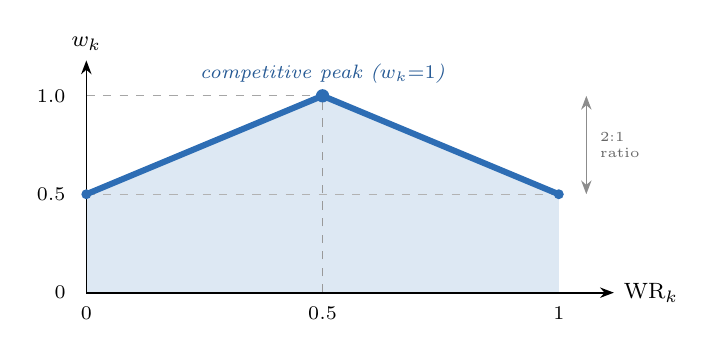
\begin{tikzpicture}[font=\small, >={Stealth[length=5pt]}]

% x: WR 0..1 -> plot x 0..6 ; y: w 0..1.0 -> plot y 0..2.5 (axis starts at 0)
% w = 1 - |WR - 0.5| in [0.5, 1.0]: peak w=1 at WR=0.5, floor w=0.5 at WR=0 and 1 (y=1.25)

%% ── shaded area under the curve ──────────────────────────────────
\fill[curvec!16] (0,0) -- (0,1.25) -- (3,2.5) -- (6,1.25) -- (6,0) -- cycle;

%% ── reference guides ─────────────────────────────────────────────
\draw[dashed, black!40] (3,0) -- (3,2.5);
\draw[dashed, black!35] (0,2.5) -- (3,2.5);
\draw[dashed, black!30] (0,1.25) -- (6,1.25);

%% ── axes ─────────────────────────────────────────────────────────
\draw[->, line width=0.6pt] (0,0) -- (6.7,0) node[right, font=\footnotesize] {$\mathrm{WR}_k$};
\draw[->, line width=0.6pt] (0,0) -- (0,2.95) node[above, font=\footnotesize] {$w_k$};

%% ── weight curve  w = 1 - |WR - 0.5| ────────────────────────────
\draw[curvec, line width=2.2pt] (0,1.25) -- (3,2.5) -- (6,1.25);
\fill[curvec] (3,2.5) circle (2.4pt);
\fill[curvec] (0,1.25) circle (1.8pt);
\fill[curvec] (6,1.25) circle (1.8pt);
\node[above=1pt, font=\scriptsize\itshape, text=curvec!82!black] at (3,2.5) {competitive peak ($w_k{=}1$)};

%% ── 2:1 range annotation (right side) ───────────────────────────
\draw[<->, black!45, line width=0.5pt] (6.35,1.25) -- (6.35,2.5);
\node[right, font=\tiny, text=black!60, align=left] at (6.4,1.875) {$2{:}1$\\ratio};

%% ── tick labels ──────────────────────────────────────────────────
\node[below, font=\scriptsize] at (0,-0.06) {$0$};
\node[below, font=\scriptsize] at (3,-0.06) {$0.5$};
\node[below, font=\scriptsize] at (6,-0.06) {$1$};
\node[left, font=\scriptsize] at (-0.14,0) {$0$};
\node[left, font=\scriptsize] at (-0.14,1.25) {$0.5$};
\node[left, font=\scriptsize] at (-0.14,2.5) {$1.0$};

\end{tikzpicture}

\end{document}
